\documentclass[twoside, openright]{report}
%% Needs to be here 
\usepackage{docstyle}
 
\title{Mall för kexjobbsrapport}
\author{Student 1
\\
Student 2}
 
\begin{document}
\maketitle
\cleardoublepage
\selectlanguage{english}
\begin{abstract}
Big wheels keep on turning\\
Carry me home to see my kin\\
Singing songs about the south-land\\
I miss 'ole' 'bamy once again and I think it's a sin\\
Well I heard Mister Young sing about her\\
Well I heard ole Neil put her down\\
Well, I hope Neil Young will remember\\
A southern man don't need him around anyhow\\
Sweet home Alabama\\
Where the skies are so blue\\
Sweet home Alabama\\
Lord, I'm coming home to you\\
In Birmingham they love the Gov'nor, boo-hoo-hoo\\
Now we all did what we could do\\
Now Watergate does not bother me\\
Does your conscience bother you, tell the truth\\
Sweet home Alabama\\
Where the skies are so blue\\
Sweet home Alabama\\
Lord, I'm coming home to you, here I come\\
Now Muscle Shoals has got the Swampers\\
And they've…\\







\end{abstract}

\cleardoublepage
\selectlanguage{swedish}
\begin{abstract}
Big wheels keep on turning\\
Carry me home to see my kin\\
Singing songs about the south-land\\
I miss 'ole' 'bamy once again and I think it's a sin\\
Well I heard Mister Young sing about her\\
Well I heard ole Neil put her down\\
Well, I hope Neil Young will remember\\
A southern man don't need him around anyhow\\
Sweet home Alabama\\
Where the skies are so blue\\
Sweet home Alabama\\
Lord, I'm coming home to you\\
In Birmingham they love the Gov'nor, boo-hoo-hoo\\
Now we all did what we could do\\
Now Watergate does not bother me\\
Does your conscience bother you, tell the truth\\
Sweet home Alabama\\
Where the skies are so blue\\
Sweet home Alabama\\
Lord, I'm coming home to you, here I come\\
Now Muscle Shoals has got the Swampers\\
And they've…\\







\end{abstract}

\newpage
\tableofcontents
\newpage

%--------------------------------
% Skriv i de separata filerna för bättre struktur
%--------------------------------

%--------------------------------
% Jag har behållit fler subsections som ni kan ta bort. Har kvar dem som inspiration
%--------------------------------

\newpage
\chapter{Introduktion}\label{chap:intro}


\section{Bakgrund}



\section{Problem}\label{sec:problem}


\section{Syfte}
Syftet med uppsatsen var att...

\section{Mål}
Arbetets mål var att...
\\\\
Uppsatsens effektmål...

\section{Fördelar, etik och hållbarhet}


\section{Metodik}
% hur ni gick tillväga, tex litteraturstudie, definiering av intressenter etc

\section{Avgränsningar}\label{sec:avgr}


\section{Disposition}
I följande kandidatuppsats finns totalt sju kapitel: 
\\\\
Kapitel ett är en introduktion till uppsatsen som berättar bakgrunden till studien och vilket problem som skulle undersökas. Kortfattat berättades det även om målet med arbete, metoder som användes och arbetets koppling till etik och hållbarhet.
\\\\
Kapitel två är en fördjupad teoretisk bakgrund till hur krav kan tas fram, vad en offert och ett offertsystem är. Det tas även upp varför agila arbetssätt är fördelaktiga och teori om utveckling av mjukvarusystem.
\\\\
Kapitel tre diskuterar och analyserar val av metoder för att genomföra projektet, samt designen av utförandet. 
\\\\
Kapitel fyra handlar om det utförda arbetet och beskriver de vetenskapliga metoder som användes för implementationen av arbetet. 
\\\\
Kapitel fem presenterar resultatet som framkom från arbetet. En översiktlig beskrivning av prototypens funktionaliteter finns.
\\\\
Kapitel sex analyserar och diskuterar resultatet, samt reflekterar över dess relation till hållbar utveckling och etik. 
\\\\ 
Kapitel sju presenterar en sammanfattning samt förslag på framtida arbete. 


\newpage
\chapter{Teori}\label{chap:teori}
Information som läsaren eventuellt inte haft sedan tidigare, som anses vara nödvändig att känna till för vidare läsning av uppsatsen, återfinns i detta kapitel. 

Exempel: Kapitlet tar först upp vad en kravspecifikation är, hur de kan tas fram och hur kraven kan se ut. Efter det följer en beskrivning av vad en offert är och de offertsystem som existerade år 2017 som Författarna kunde ta lärdom av. Kapitlet beskriver även modeller som använts för själva arbetsproceduren samt prototypen. Sist presenteras vad ett ramverk är och varför arbetet krävde ett. 

\section{Kravspecifikation}

\subsubsection{Kravframställning} 

\paragraph{Workshop}

\paragraph{Intervjutekniker}

\subsubsection{Modellering- och analyseringskrav}


\subsubsection{Kommunikationskrav}


\subsubsection{Överenskommelsekrav}


\subsubsection{Utvecklingskrav}


\section{En offert}\label{sec:offert}
% vad innebär denna term som kommer att användas i arbetet

\subsection{Ett offertsystem}
% vad är ett offertsystem

\section{Modeller för systemutveckling}

\subsection{Arbetsmodell}
% vattenfall vs agil

\subsection{Prototyputveckling}




\section{Ramverk}
% varför det behövdes

\section{Modellering av en verksamhet}
%beskriver hur man modellerar en verksamhet

\newpage
\chapter{Metoder}\label{chap:metod}

 
\section{Litteraturstudie}
%hur litteraturstudien gick till och vad resultaten från den var

\section{Prototyp}
% tex prototyp av evolutionär karaktär

\section{Arbetsmetod}
% tex agil

\section{Kravframtagning}

\paragraph{Workshop}
% varför workshop, tillvägagångssätt etc.


\paragraph{Intervjuer}
% varför det var en lämplig teknik, tillvägagångssätt etc 



\section{Utvecklingsmiljö}
% tex val av databas




\newpage
\chapter{Arbetet}\label{chap:arbete}
För att kunna nå fram till resultatet genomfördes...

\section{Kravframställning och verksamhetsmodellering}\label{sec:arbkrav}

\subsection{Klassmodell}
Exempel på insert av figur
\begin{figure}[!ht]
\centering
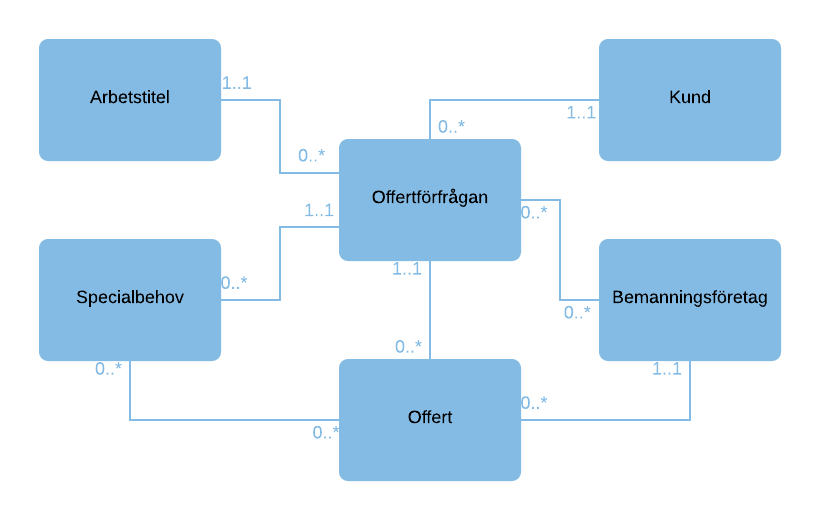
\includegraphics[width=1\textwidth]{fig/Klassmodelll.png}
\caption{\label{fig:klassModell}Klassmodell av offertsystemet.}
\end{figure}


\section{Modellering och design av databas}

\section{Utveckling av MVP version av applikationen}\label{sec:arbmvp}




\newpage
\chapter{Resultat}\label{chap:result}
Skriv om resultatet








\newpage
\chapter{Diskussion}\label{chap:diss}
Exempel på rubriker


\section{Insamling av krav}


\section{Arbetsmetod}


\section{Testning}


\section{Hållbar utveckling och etik}

  

\newpage
\chapter{Sammanfattning och framtida arbete}\label{chap:SamFut}
I sista kapitlet beskrivs resultatet i en sammanfattning och framtida arbete presenteras.

\section{Sammanfattning}


\section{Framtida arbete}

  

\newpage
\addcontentsline{toc}{chapter}{Litteraturförteckning}
\printbibliography[title=Litteraturförteckning]

\newpage
\begin{appendices}
\addtocontents{toc}{\protect\setcounter{tocdepth}{0}}
  \chapter{Titel till appendix}
    \section{Första sektionen}\label{sek:exempel2}
  Big wheels keep on turning\\
Carry me home to see my kin\\
Singing songs about the south-land\\
I miss 'ole' 'bamy once again and I think it's a sin\\
Well I heard Mister Young sing about her\\
Well I heard ole Neil put her down\\
Well, I hope Neil Young will remember\\
A southern man don't need him around anyhow\\
Sweet home Alabama\\
Where the skies are so blue\\
Sweet home Alabama\\
Lord, I'm coming home to you\\
In Birmingham they love the Gov'nor, boo-hoo-hoo\\
Now we all did what we could do\\
Now Watergate does not bother me\\
Does your conscience bother you, tell the truth\\
Sweet home Alabama\\
Where the skies are so blue\\
Sweet home Alabama\\
Lord, I'm coming home to you, here I come\\
Now Muscle Shoals has got the Swampers\\
And they've…\\







  \section{Andra sektionen}\label{sek:exempel2}
  Big wheels keep on turning\\
Carry me home to see my kin\\
Singing songs about the south-land\\
I miss 'ole' 'bamy once again and I think it's a sin\\
Well I heard Mister Young sing about her\\
Well I heard ole Neil put her down\\
Well, I hope Neil Young will remember\\
A southern man don't need him around anyhow\\
Sweet home Alabama\\
Where the skies are so blue\\
Sweet home Alabama\\
Lord, I'm coming home to you\\
In Birmingham they love the Gov'nor, boo-hoo-hoo\\
Now we all did what we could do\\
Now Watergate does not bother me\\
Does your conscience bother you, tell the truth\\
Sweet home Alabama\\
Where the skies are so blue\\
Sweet home Alabama\\
Lord, I'm coming home to you, here I come\\
Now Muscle Shoals has got the Swampers\\
And they've…\\








\end{appendices}

\end{document}